\documentclass[11pt]{article}

\usepackage[margin=1in]{geometry}
\usepackage{amsmath,amssymb,amsthm}
\usepackage{booktabs}
\usepackage{graphicx}
\usepackage{hyperref}
\usepackage{placeins}
\usepackage{xurl}
\usepackage[numbers,sort&compress]{natbib}
\usepackage{xcolor}

\graphicspath{{../figures/}}
\hypersetup{hidelinks}
\urlstyle{same}
\emergencystretch=3em
\makeatletter
\setlength{\@fptop}{0pt}
\makeatother

\newtheorem{theorem}{Theorem}
\newtheorem{proposition}{Proposition}
\newtheorem{definition}{Definition}
\newtheorem{assumption}{Assumption}

\title{Prediction Uncertainty Is Not Control Risk:\\
Counterfactual Risk Calibration for Learned-Dynamics MPC}
\author{Anonymous Authors}
\date{}

\begin{document}
\maketitle

\begin{abstract}
Learned dynamics models are often evaluated by one-step prediction error, predictive uncertainty, or prediction calibration. Model-predictive control (MPC), however, uses a learned model to choose an action. A planner therefore needs a decision-level object: whether plausible learned dynamics models make different candidate trajectories low-regret, unsafe, or rank-preferred. We study this distinction in a bounded CPU-reproducible suite of simplified learned-dynamics MPC tasks. We define counterfactual control risk (CCR), a candidate-level score built from regret, violation tails, constraint-margin tails, rank instability, and first-action disagreement across dynamics particles. A split calibration layer maps CCR scores to observed planned-trajectory failures, and CCR-MPC selects the lowest-cost sampled candidate that passes calibrated risk gates. Across six simplified domains, nineteen methods/ablations, three OOD shift levels, and seeds 0,1,2, CCR-MPC reduced mean closed-loop violation rate from 1.14\% for vanilla MPPI to 0.42\%, with mean cost 29.41 versus 28.47 for vanilla MPPI and 28.54 for oracle MPC. CCR-MPC tied the lowest aggregate violation rate of CVaR/RA-MPPI and conformal-prediction MPC in this suite, but did not dominate them in cost. The supported claim is therefore bounded: prediction uncertainty alone is an incomplete proxy for control risk, and calibrated counterfactual decision features can improve safety over vanilla and uncalibrated learned-dynamics MPC in these simplified sampled-planning settings. The experiments do not establish hardware safety or broad robotics generality.
\end{abstract}

\section{Introduction}

Learned dynamics models are central to model-based reinforcement learning and model-predictive control. Work on probabilistic dynamics and world models has made prediction-space uncertainty useful for sample-efficient control \citep{chua2018pets,hafner2020dreamer,lakshminarayanan2017deepensembles}. Sampling-based MPC methods such as MPPI and information-theoretic MPC can then optimize nonlinear costs online using learned or simulated dynamics \citep{williams2017mppi,williams2017itm}. Yet a planner ultimately chooses an action. Prediction uncertainty is relevant only through its effect on that choice.

This paper asks a narrower question: when a learned dynamics ensemble is prediction-calibrated or low-error, is its uncertainty automatically calibrated for closed-loop control risk? The answer is no. A model can be accurate on the prediction distribution while small model differences near a constraint boundary flip the action selected by MPC. In that regime, the risk object is not simply the spread of predicted next states. It is whether plausible models make a candidate trajectory high-regret, constraint-violating, or decision-unstable.

We introduce \emph{counterfactual control risk} (CCR), a planner-level statistic over sampled candidate action sequences. Given dynamics particles and a candidate set, CCR measures regret relative to each particle's own preferred candidate, violation and margin tails, rank instability, and first-action disagreement. CCR-MPC then calibrates these scores on held-out candidate contexts and uses them as a risk gate inside MPC/MPPI.

The contribution is intentionally scoped:
\begin{itemize}
  \item We give a constructive separation theorem showing why prediction calibration or low prediction error need not imply control-risk calibration.
  \item We define CCR features and a split-calibrated CCR-MPC selection rule for sampled learned-dynamics MPC.
  \item We execute a CPU-reproducible simplified suite with nineteen methods and ablations, including vanilla MPPI, robust MPC, CVaR/RA-MPPI-style control, conformal non-CCR baselines, uncertainty penalties, system-ID proxy, domain-randomized MPC, oracle MPC, and single-feature ablations.
  \item We report where the method helps and where it does not: CCR-MPC improves violation rate over vanilla MPPI and uncalibrated CCR in the generated suite, but it ties rather than beats the strongest CVaR and conformal-prediction baselines on aggregate violation rate.
\end{itemize}

\section{Problem Setup}

Let $x_t \in \mathcal{X}$ denote the state, $u_t \in \mathcal{U}$ the action, and $f^\star$ the true closed-loop dynamics. The controller has access to a finite set of learned dynamics particles
\[
  \mathcal{F} = \{f_1,\ldots,f_K\},
\]
obtained from bootstrapping, posterior sampling, dropout particles, perturbations, or simplified learned-model surrogates. At each planning step, the planner samples candidate action sequences
\[
  \mathcal{U}_H = \{U_1,\ldots,U_N\}, \qquad U_j=(u_{j,0},\ldots,u_{j,H-1}).
\]
Rolling out candidate $U_j$ under particle $f_i$ gives a predicted cost $J_i(U_j)$, a violation indicator $V_i(U_j)\in\{0,1\}$, and a minimum constraint margin $M_i(U_j)$, where negative margin indicates predicted violation.

The planner executes only the first action of the selected sequence, then replans. The evaluation metric is closed-loop violation frequency and task cost under $f^\star$.

\begin{definition}[Prediction risk versus control risk]
Prediction risk is a loss on model outputs, such as one-step error or calibrated prediction-set coverage. Control risk is a loss on the action selected by a planner using the model, such as closed-loop constraint violation or regret against an oracle dynamics planner.
\end{definition}

The paper studies the gap between these two quantities for sampled learned-dynamics MPC.

\section{Counterfactual Control Risk}

For each dynamics particle, define the particle-optimal sampled candidate
\[
  U_i^\star \in \arg\min_{U\in\mathcal{U}_H} J_i(U).
\]
The counterfactual regret of candidate $U_j$ under particle $f_i$ is
\[
  R_{ij} = J_i(U_j) - J_i(U_i^\star).
\]
This regret is counterfactual because it asks: if particle $f_i$ were the dynamics model trusted by the planner, how much worse would $U_j$ be than the candidate that particle would have preferred?

\subsection{CCR Features}

The implementation uses the following candidate-level features:
\begin{align}
  \phi_{\mathrm{regret}}(U_j) &= \mathrm{CVaR}_q(\{R_{ij}\}_{i=1}^K),\\
  \phi_{\mathrm{viol}}(U_j) &= \frac{1}{K}\sum_i V_i(U_j),\\
  \phi_{\mathrm{tail}}(U_j) &= \mathrm{CVaR}_q(\{V_i(U_j)\}_{i=1}^K),\\
  \phi_{\mathrm{margin}}(U_j) &= \mathrm{CVaR}_q(\{\max(0,-M_i(U_j))\}_{i=1}^K).
\end{align}
It also computes rank instability across particles and first-action disagreement. The combined CCR score is a normalized weighted sum. The weights used in the generated CPU study are recorded in \texttt{skeleton/ccr\_mpc.py} and \texttt{scripts/execute\_paper\_cpu\_study.py}.

\subsection{Split Calibration}

Calibration data consists of candidate contexts $(x,\mathcal{U}_H,\mathcal{F})$ with observed candidate failure labels under the true simulator. For a scalar score $S(U)$, the calibrator sorts calibration candidates by score and estimates the accepted-candidate failure rate for each threshold. It selects the largest threshold whose one-sided concentration upper bound is at most the target risk $\alpha$.

At test time, CCR-MPC uses calibrated gates on combined CCR, predicted violation, and negative margin tail. Among candidates passing the gates, it selects the lowest adjusted cost. If no candidate passes, it selects the candidate with minimum calibrated risk plus a small cost-normalized tie-breaker.

\paragraph{Algorithm.}
At each MPC step:
\begin{enumerate}
  \item sample $N$ action sequences around a local feedback proposal;
  \item evaluate each sequence under $K$ dynamics particles;
  \item compute $J_i(U_j)$, $V_i(U_j)$, $M_i(U_j)$, and CCR features;
  \item apply split-calibrated CCR/violation/margin thresholds;
  \item execute the first action of the lowest adjusted-cost accepted candidate, or the minimum-risk fallback candidate if none is accepted.
\end{enumerate}

\section{Theory}

The theory is intentionally narrow. It formalizes the proxy gap for a sampled one-step MPC problem and states the finite-threshold calibration guarantee used by the implementation. It does not prove broad robotics safety.

\begin{theorem}[Prediction error on the data distribution need not control MPC risk]
For any $\epsilon>0$ and any $\rho\in(0,1]$, there exists a deterministic constrained one-dimensional control problem, a training distribution $\mathcal{D}$, an evaluation distribution $\mathcal{E}$, two learned dynamics models $f_a,f_b$, and a two-candidate one-step MPC planner such that the one-step prediction losses of $f_a$ and $f_b$ on $\mathcal{D}$ differ by at most $\epsilon$, yet the planner using $f_a$ has zero violation probability on $\mathcal{E}$ while the planner using $f_b$ has violation probability at least $\rho$.
\end{theorem}

\begin{proof}
Let the true dynamics be $f^\star(x,u)=x+u$ and impose the one-step safety constraint $x^+\leq 0$. Choose $\eta>0$ and the evaluation state $x_0=-\eta/2$. The candidate set contains $u_s=-\eta/2$ and $u_r=\eta$. Under the true dynamics, $u_s$ gives $x^+=-\eta$ and is safe, while $u_r$ gives $x^+=\eta/2$ and violates the constraint.

Let the planner minimize the predicted one-step objective
\[
  (f(x,u))^2 + \lambda \mathbf{1}\{f(x,u)>0\},
\]
with $\lambda>\eta^2$. Define $f_a=f^\star$. Define $f_b=f^\star$ outside the boundary neighborhood $B=[-\eta,0]$ and $f_b(x,u)=f^\star(x,u)-\eta$ for $x\in B$. Put all mass of the training distribution $\mathcal{D}$ outside $B$. Then $f_a$ and $f_b$ have identical one-step loss on $\mathcal{D}$, so their loss difference is $0\leq\epsilon$.

At $x_0$, the planner using $f_a$ penalizes $u_r$ as unsafe and chooses $u_s$. The planner using $f_b$ predicts $u_s$ as $-2\eta$ and $u_r$ as $-\eta/2$, so both candidates are predicted safe and $u_r$ is closer to the target boundary $0$; it chooses $u_r$. Let $\mathcal{E}$ place probability $\rho$ on $x_0$ and the remaining mass on states where both planners choose safe actions. The violation-risk gap on $\mathcal{E}$ is therefore at least $\rho$. Thus equal prediction loss on the training distribution does not imply equal MPC-induced control risk under the evaluation distribution.
\end{proof}

\begin{assumption}[Exchangeable candidate contexts]
Calibration and test candidate contexts are exchangeable after conditioning on the declared domain, OOD level, candidate-generation rule, and dynamics-particle construction.
\end{assumption}

\begin{proposition}[Finite-threshold split CCR risk control]
Let $(S_i,Y_i)_{i=1}^m$ be exchangeable calibration examples, where $S_i$ is a scalar CCR score and $Y_i\in\{0,1\}$ is a candidate-failure label. Let $\mathcal{T}$ be a finite set of thresholds and let lower scores be accepted. For $\tau\in\mathcal{T}$, define $n_\tau=\sum_i\mathbf{1}\{S_i\leq\tau\}$ and
\[
  \widehat p_\tau = \frac{1}{n_\tau}\sum_{i:S_i\leq\tau} Y_i
\]
when $n_\tau>0$. If CCR-MPC chooses a threshold $\widehat\tau$ satisfying
\[
  \widehat p_{\widehat\tau} +
  \sqrt{\frac{\log(2|\mathcal{T}|/\delta)}{2n_{\widehat\tau}}}
  \leq \alpha,
\]
then, with probability at least $1-\delta$ over the split calibration sample, the failure probability of a fresh exchangeable accepted candidate under $\widehat\tau$ is at most $\alpha$ for all thresholds whose accepted examples obey the bounded-label sampling model.
\end{proposition}

\begin{proof}
For any fixed $\tau$ with $n_\tau>0$, the accepted labels are bounded Bernoulli variables drawn from the conditional population $\{Y:S\leq\tau\}$. Hoeffding's inequality gives
\[
  \Pr\left(p_\tau >
  \widehat p_\tau +
  \sqrt{\frac{\log(2|\mathcal{T}|/\delta)}{2n_\tau}}\right)
  \leq \frac{\delta}{|\mathcal{T}|},
\]
where $p_\tau=\Pr(Y=1\mid S\leq\tau)$. A union bound over $\mathcal{T}$ gives simultaneous validity for all finite thresholds with probability at least $1-\delta$. Since $\widehat\tau$ is selected from this same finite set using only split calibration labels, the simultaneous bound applies to the selected threshold. The stated threshold condition then implies $p_{\widehat\tau}\leq\alpha$.
\end{proof}

\begin{proposition}[Sampled safe-cost optimality]
Conditioned on a sampled candidate set and a calibrated accepted set $\mathcal{A}$, CCR-MPC selects a candidate whose adjusted predicted cost is no greater than any other candidate in $\mathcal{A}$. The gap to the best continuous-control safe trajectory is the sum of candidate-sampling error, model-prediction error, and calibration-threshold error.
\end{proposition}

\begin{proof}
If $\mathcal{A}$ is nonempty, the implementation returns an element of $\arg\min_{U\in\mathcal{A}}\widetilde J(U)$, where $\widetilde J$ is the adjusted predicted cost used by the planner. The first claim follows directly from the definition of the argmin. Any comparison to an unsampled continuous-control trajectory must pass through three approximations: whether the candidate sampler included a near-optimal safe sequence, whether $\widetilde J$ preserves the true safe-cost ordering, and whether the calibrated threshold accepts that sequence. These are exactly the candidate-sampling, model-prediction, and calibration-threshold terms; no stronger global optimality claim is made.
\end{proof}

\section{Experiments}

\subsection{Domains and Budget}

The generated suite uses six simplified CPU domains: synthetic separation, constrained double-integrator, lateral car surrogate, planar-quadrotor altitude surrogate, quasi-static pushing surrogate, and a CEM-MPC secondary-planner setting. These are not high-fidelity simulators. They are controlled low-dimensional environments designed to expose decision sensitivity under learned dynamics shift.

The focused run uses 1026 closed-loop runs and 20862 planning-step predictions: six domains, nineteen methods/ablations, three OOD levels, and seeds 0,1,2. Candidate budget is 32 sequences per planning step in the focused run, with seven learned dynamics particles unless a method definition uses oracle, system-ID proxy, or domain-randomized particles. Calibration uses 36 sampled contexts per domain/OOD pair. The target risk parameter is $\alpha=0.15$. The recorded execution environment is Windows 10 on an AMD64 machine with an Intel64-family processor and Python 3.10.11; the focused run took 216.9 seconds.

\subsection{Baselines}

Baselines include vanilla MPPI, robust MPC, raw ensemble uncertainty penalty, prediction-calibrated uncertainty penalty, CVaR/RA-MPPI-style control \citep{yin2023ramppi}, chance-constrained MPC, conformal prediction MPC, non-CCR conformal risk, and a conformal decision baseline \citep{angelopoulos2024conformalrisk,lekeufack2023conformaldecision}. The suite also includes a SODA-like uncertainty fallback, domain-randomized MPC, system-ID proxy MPC, oracle MPC, and CCR ablations.

\subsection{Metrics}

We report mean episode cost, mean closed-loop violation rate, episode-level observed risk, calibration metrics (ECE, Brier, log loss), freezing rate, fallback rate, mean planning time per step, oracle regret, and mean prediction error. Raw logs are stored under \path{logs/}.

\begin{table}[t]
\centering
\scriptsize
\begin{tabular}{lccccc}
\toprule
Method & Cost & Viol. \% & Obs. \% & Freeze \% & ms/step \\
\midrule
Vanilla MPPI & 28.47 (1.82) & 1.14 (0.47) & 12.96 (4.61) & 14.84 (1.63) & 7.47 (0.09) \\
Robust MPC & 28.69 (1.82) & 0.51 (0.29) & 7.41 (3.60) & 14.73 (1.28) & 7.64 (0.10) \\
CVaR/RA-MPPI & 28.65 (1.82) & 0.42 (0.28) & 5.56 (3.15) & 15.39 (1.50) & 8.33 (0.08) \\
Conf. prediction MPC & 29.67 (1.83) & 0.42 (0.28) & 5.56 (3.15) & 19.69 (3.06) & 8.61 (0.10) \\
Conf. risk, non-CCR & 28.55 (1.81) & 0.51 (0.29) & 7.41 (3.60) & 15.64 (1.71) & 8.50 (0.10) \\
CCR no calibration & 28.86 (1.82) & 1.12 (0.46) & 12.96 (4.61) & 13.94 (1.25) & 7.43 (0.09) \\
CCR-MPC & 29.41 (1.86) & 0.42 (0.28) & 5.56 (3.15) & 12.46 (1.27) & 10.47 (0.10) \\
Oracle MPC & 28.54 (1.82) & 0.63 (0.34) & 7.41 (3.60) & 15.32 (1.53) & 6.98 (0.08) \\
\bottomrule

\end{tabular}
\caption{Focused CPU run. Entries are mean (SEM) over 54 domain/OOD/seed runs per method; percentage SEMs are in percentage points. CCR-MPC reduces violation rate relative to vanilla MPPI and uncalibrated CCR, and matches the lowest aggregate violation rate in this suite. It does not dominate CVaR/RA-MPPI or conformal-prediction MPC in cost, so the supported conclusion is a bounded safety-performance tradeoff rather than broad superiority.}
\label{tab:main}
\end{table}

\begin{table}[t]
\centering
\small
\begin{tabular}{lrrrr}
\toprule
Ablation & Cost & Viol. rate & Freeze & Oracle regret \\
\midrule
CCR-MPC & 29.41 & 0.42\% & 12.46\% & 0.87 \\
CCR no calibration & 28.86 & 1.12\% & 13.94\% & 0.32 \\
Calibration no CCR & 45.08 & 5.36\% & 42.05\% & 16.55 \\
Disagreement only & 33.32 & 3.60\% & 31.24\% & 4.78 \\
Regret only & 38.91 & 0.42\% & 36.32\% & 10.37 \\
Violation tail only & 49.88 & 0.42\% & 75.16\% & 21.35 \\
\bottomrule
\end{tabular}
\caption{Ablations. Single-feature conservative gates can match CCR-MPC's violation rate, but at much higher cost and freezing. This supports the combined-score design only within the simplified suite; it does not prove the weights are optimal.}
\label{tab:ablation}
\end{table}

\subsection{Results and Interpretation}

Table~\ref{tab:main} shows the main aggregate result. CCR-MPC reduces mean violation rate from 1.14\% for vanilla MPPI to 0.42\%, and from 1.12\% for uncalibrated CCR to 0.42\%. Its observed episode-level failure rate is 5.56\%, compared with 12.96\% for vanilla and uncalibrated CCR. The cost increases from 28.47 to 29.41 relative to vanilla.

The strongest caveat is visible in the same table: CVaR/RA-MPPI also attains 0.42\% mean violation rate with lower mean cost, and conformal-prediction MPC attains the same violation rate with slightly higher cost. The violation-rate SEM for the low-violation tier is 0.28 percentage points, so the aggregate tie should be read as a bounded matched-safety result rather than a statistically separated ranking among these methods. Thus the result does not support a claim that CCR-MPC is uniformly better than risk-aware or conformal alternatives. The supported claim is that CCR features plus calibration provide a useful decision-risk layer relative to vanilla and uncalibrated CCR in this controlled suite.

Table~\ref{tab:ablation} shows that single-feature conservative gates can match the violation rate but often freeze or pay much larger cost. The violation-tail-only baseline reaches 0.42\% violation rate but with cost 49.88 and freezing 75.16\%. The regret-only baseline also reaches 0.42\% but with cost 38.91. CCR-MPC preserves a lower cost while using a combined decision-risk score.

\begin{figure}[t]
\centering
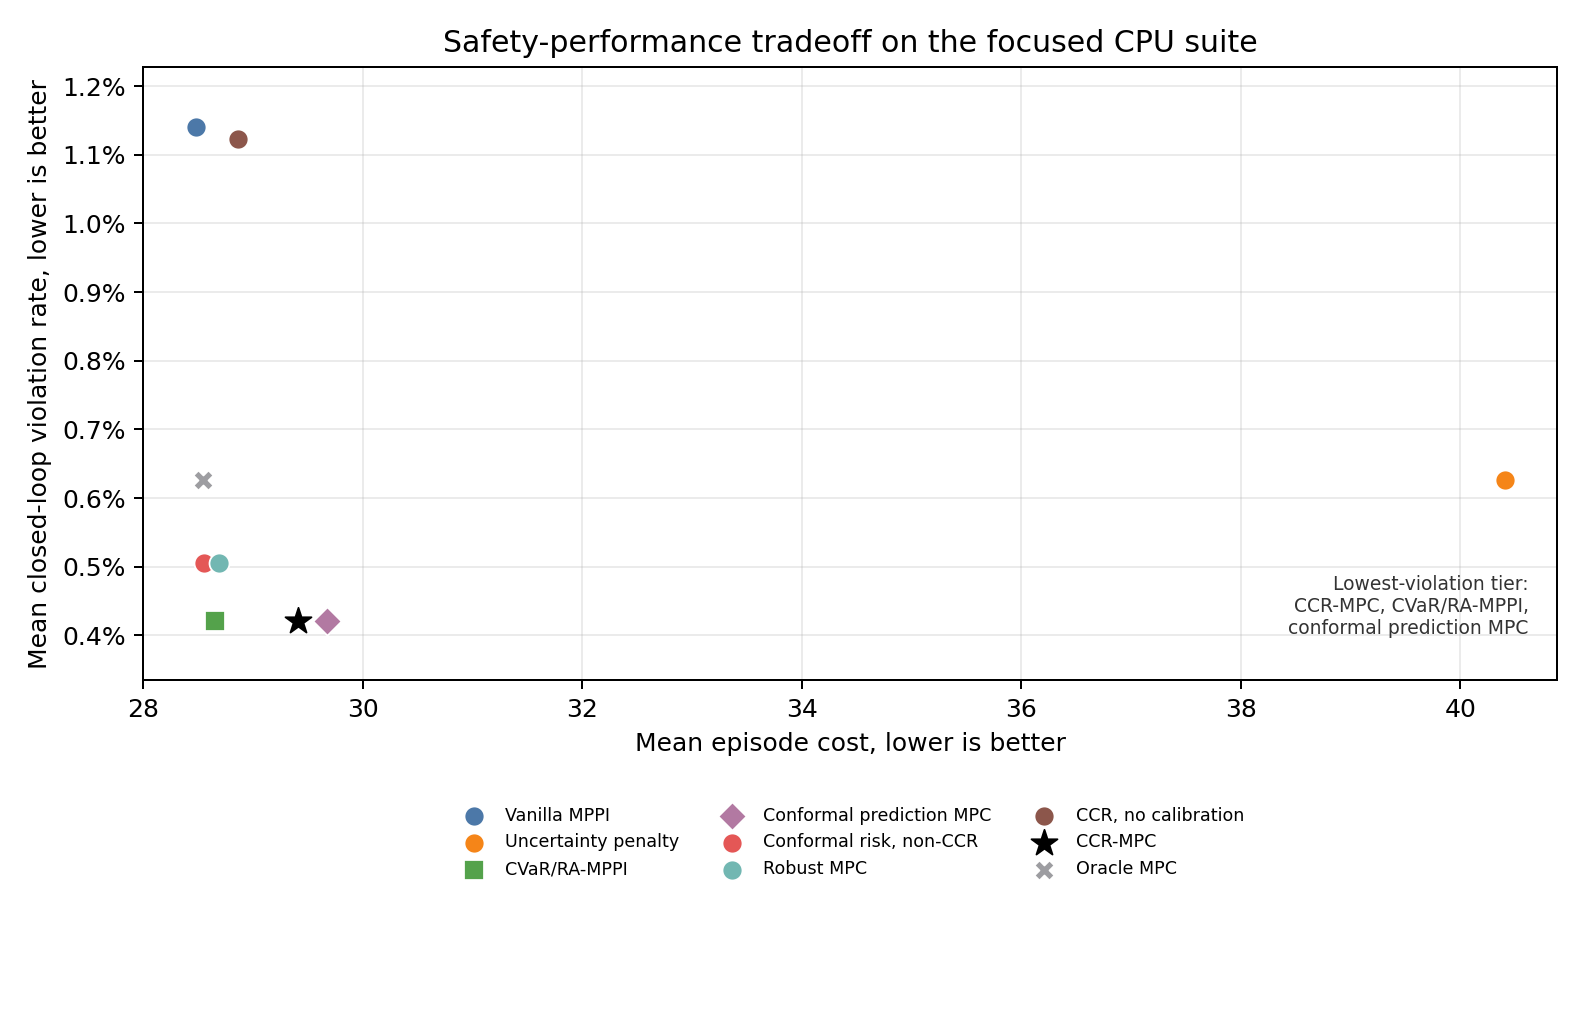
\includegraphics[width=0.85\linewidth]{safety_performance_pareto.png}
\caption{Safety-performance tradeoff across important methods. Axes are mean episode cost and mean closed-loop violation rate over the focused CPU suite. CCR-MPC sits in the low-violation region but is not the lowest-cost low-violation method.}
\label{fig:pareto}
\end{figure}

\begin{figure}[t]
\centering
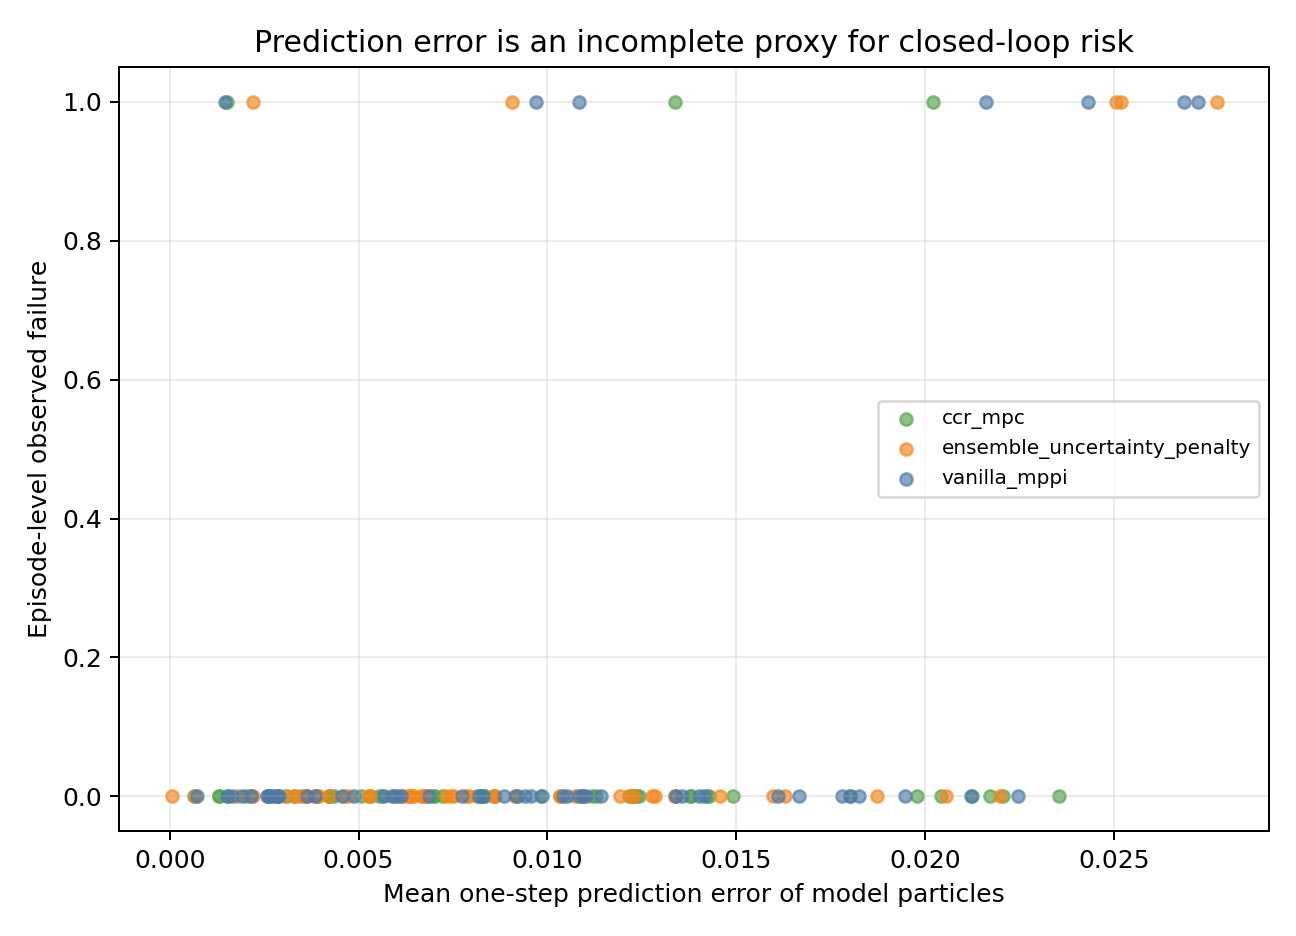
\includegraphics[width=0.75\linewidth]{prediction_error_vs_control_risk.png}
\caption{Prediction error versus episode-level control failure. The plot is intended as evidence for the proxy gap: prediction error alone does not determine whether the selected closed-loop action sequence fails.}
\label{fig:predrisk}
\end{figure}

\begin{figure}[t]
\centering
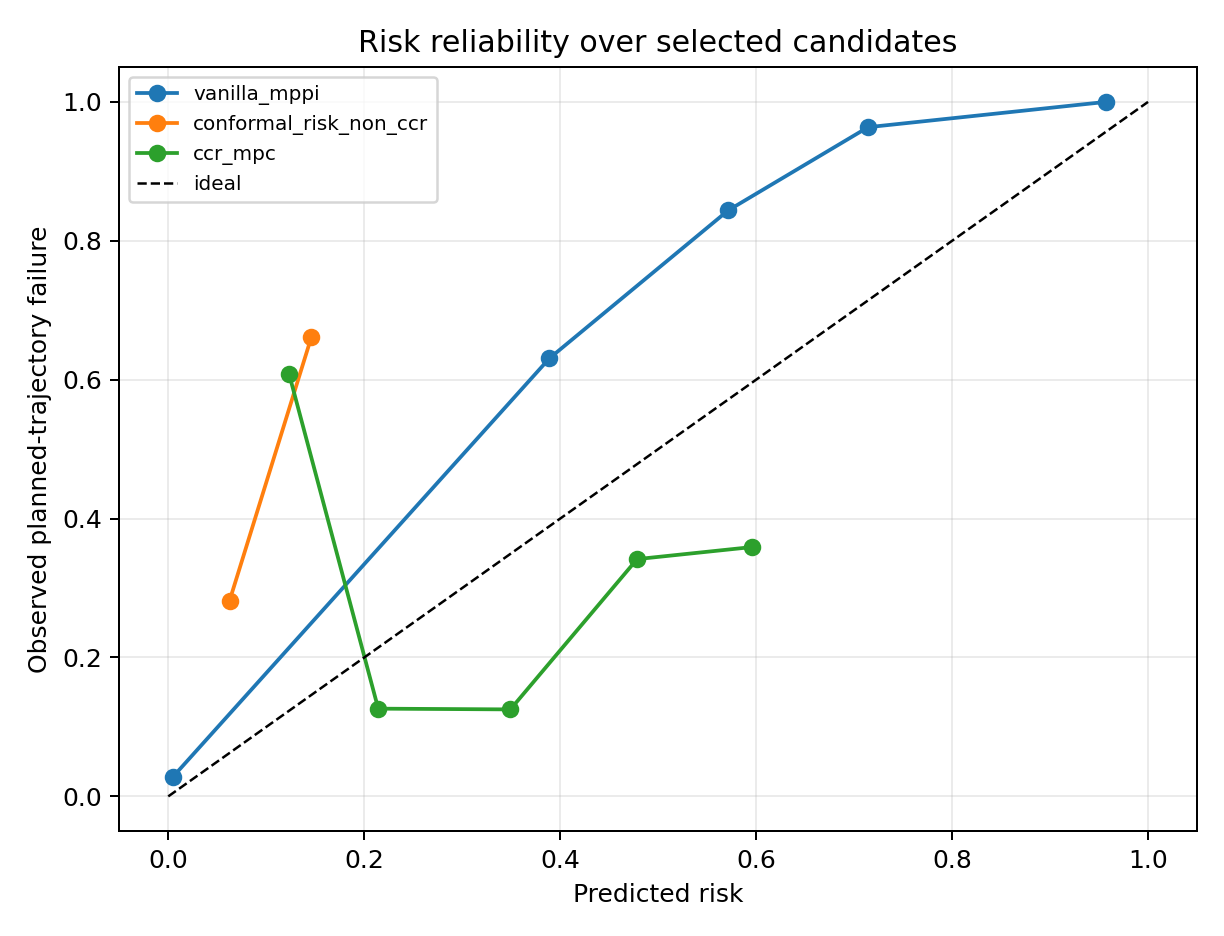
\includegraphics[width=0.75\linewidth]{risk_reliability.png}
\caption{Reliability of predicted candidate risk against planned-trajectory failure. This figure should be interpreted within the simplified calibration/evaluation distribution only.}
\label{fig:reliability}
\end{figure}

\FloatBarrier

\section{Related Work}

\paragraph{Learned dynamics and model-based control.}
Probabilistic dynamics ensembles and model-based RL methods use model uncertainty to improve sample efficiency and planning \citep{chua2018pets,lakshminarayanan2017deepensembles,hafner2020dreamer}. Sampling-based MPC and MPPI optimize candidate trajectories online under nonlinear dynamics and costs \citep{williams2017mppi,williams2017itm}. CCR-MPC keeps this sampled-planning structure but changes the risk statistic from prediction spread to decision instability and counterfactual regret.

\paragraph{Risk-aware MPC and robust MPC.}
Robust MPC and scenario MPC reason about constraint satisfaction under uncertainty sets or sampled scenarios \citep{mayne2005robustmpc,calafiore2013scenario}. Learning-based MPC methods combine data-driven model improvement with safety or robustness assumptions \citep{aswani2013lbmpc,koller2018safeexploration}. RA-MPPI uses CVaR to bias sampling-based control toward lower tail risk \citep{yin2023ramppi}. In our generated suite, CVaR/RA-MPPI is a strong baseline that ties CCR-MPC in aggregate violation rate and has lower mean cost. The distinction is therefore conceptual rather than empirical dominance: CCR estimates planner-instability risk across plausible learned models, while CVaR optimizes an upper-tail cost/violation objective.

\paragraph{Conformal prediction and decision calibration.}
Conformal prediction gives distribution-free predictive sets under exchangeability \citep{angelopoulos2023gentle}. Conformal risk control extends this perspective to monotone losses \citep{angelopoulos2024conformalrisk}, and conformal decision theory calibrates decisions directly \citep{lekeufack2023conformaldecision}. Conformal prediction has also been used for safe planning in dynamic environments \citep{lindemann2023safeplanning}. CCR-MPC is closest to conformal risk/decision calibration, but contributes a control-specific score based on counterfactual sampled-planner regret, margins, and action/rank instability. The generated experiments include non-CCR conformal baselines precisely because the novelty is the score and its planner-level interpretation, not the general idea of split calibration.

\section{Limitations}

The limitations are material. First, the experiments are simplified two-state CPU surrogates, not high-fidelity robot or hardware experiments. Second, the dynamics particles are synthetic learned-model surrogates rather than neural dynamics models trained from raw robot datasets. Third, the theory is limited to a stylized one-step separation, finite-threshold split calibration, and optimality over sampled accepted candidates; it does not cover adaptive online distribution shift or continuous-control global optimality. Fourth, the exchangeability assumption for calibration is fragile under online distribution shift. Fifth, the focused run executes 1026 closed-loop runs, not the full 57000-row max-out matrix. Sixth, CCR-MPC does not dominate CVaR/RA-MPPI or conformal-prediction MPC in the focused suite. These limitations should remain in the abstract, results interpretation, and reviewer response.

\section{Reproducibility}

The package contains all generated artifacts. The focused run can be reproduced with:
\begin{verbatim}
python scripts/execute_paper_cpu_study.py --profile focused \
  --seeds 0,1,2 --candidates 32 --calibration-contexts 36
\end{verbatim}
The main raw logs are results.jsonl, results\_flat.csv, and step\_predictions.csv in the logs directory. The manifest \path{reports/final_artifact_manifest.json} records hashes for code, logs, figures, tables, reports, and this manuscript.

\section{Conclusion}

Prediction uncertainty is useful but incomplete for learned-dynamics MPC. A sampled planner needs to know whether plausible models change which candidate is low-regret or unsafe. CCR operationalizes this decision-level risk by measuring counterfactual regret, violation tails, margins, and instability across dynamics particles, then calibrating those features to observed candidate failures. In the generated simplified CPU suite, CCR-MPC improves safety over vanilla MPPI and uncalibrated CCR at moderate cost, while tying rather than surpassing the strongest CVaR and conformal-prediction baselines. The current evidence supports a bounded decision-calibration claim and motivates stronger future validation in richer learned dynamics and robot simulation settings.

\bibliographystyle{plainnat}
\bibliography{references}

\appendix
\section{Artifact Map}

Code artifacts are under the scripts and skeleton directories. Logs include the JSONL result log, the flat run table, step-level predictions, and calibration samples. Tables include the method summary, domain/method summary, method/level summary, and generated LaTeX rows used by Table~\ref{tab:main}. Figures and reports are under the figures and reports directories; the manifest records exact paths and hashes.

\section{Full Method List}

MPC and risk baselines are vanilla MPPI, robust MPC, CVaR/RA-MPPI-style control, chance-constrained MPC, domain-randomized MPC, system-ID proxy MPC, oracle MPC, and SODA-like fallback. Calibration and conformal baselines are ensemble uncertainty penalty, prediction-calibrated penalty, conformal prediction MPC, non-CCR conformal risk, and conformal decision baseline. CCR ablations are CCR without calibration, calibration without CCR, disagreement only, regret only, violation tail only, and CCR-MPC.

\end{document}
